\large
\section{Electrons}
\label{sec:electron}
When an high energy electron (or positron) enters the detector, 
it interacts with the detector material primarily via bremsstrahlung. 
This results in radiation of photons, which subsequently convert into 
electron–positron pairs that continue to 
interact with the detector material, 
leading to a cascade of particles of decreasing energy.
These cascade particles are usually referred to as electromagnetic \textit{shower}.
They are very collimated and frequently create 
neighbouring signals in the calorimeter component. 
% as part of the same electromagnetic cluster. 
These interactions can occur inside the ID volume 
or even in the beam pipe, generating multiple tracks
in the ID, or can instead occur downstream 
of the ID, only impacting the shower in
the calorimeter. 
\subsection{Reconstruction}
% Therefore, it is possible to produce and match multiple tracks to the same electromagnetic
% cluster, all originating from the same primary electron.
The reconstruction of electron is based on three fundamental components: 
a) localised clusters of energy deposits found within the EM calorimeter, 
b) charged tracks identified in the ID (as described in details in chapter~\ref{sec:track}),
and c) close matching in $\eta \times \phi$ space of the tracks to the clusters~\cite{PERF-2017-01}.
Figure~\ref{fig:electron_recon} provides a schematic illustration of the elements that enter into
the reconstruction and identification of an electron. 
\begin{figure}[bht]
    \begin{centering}	
    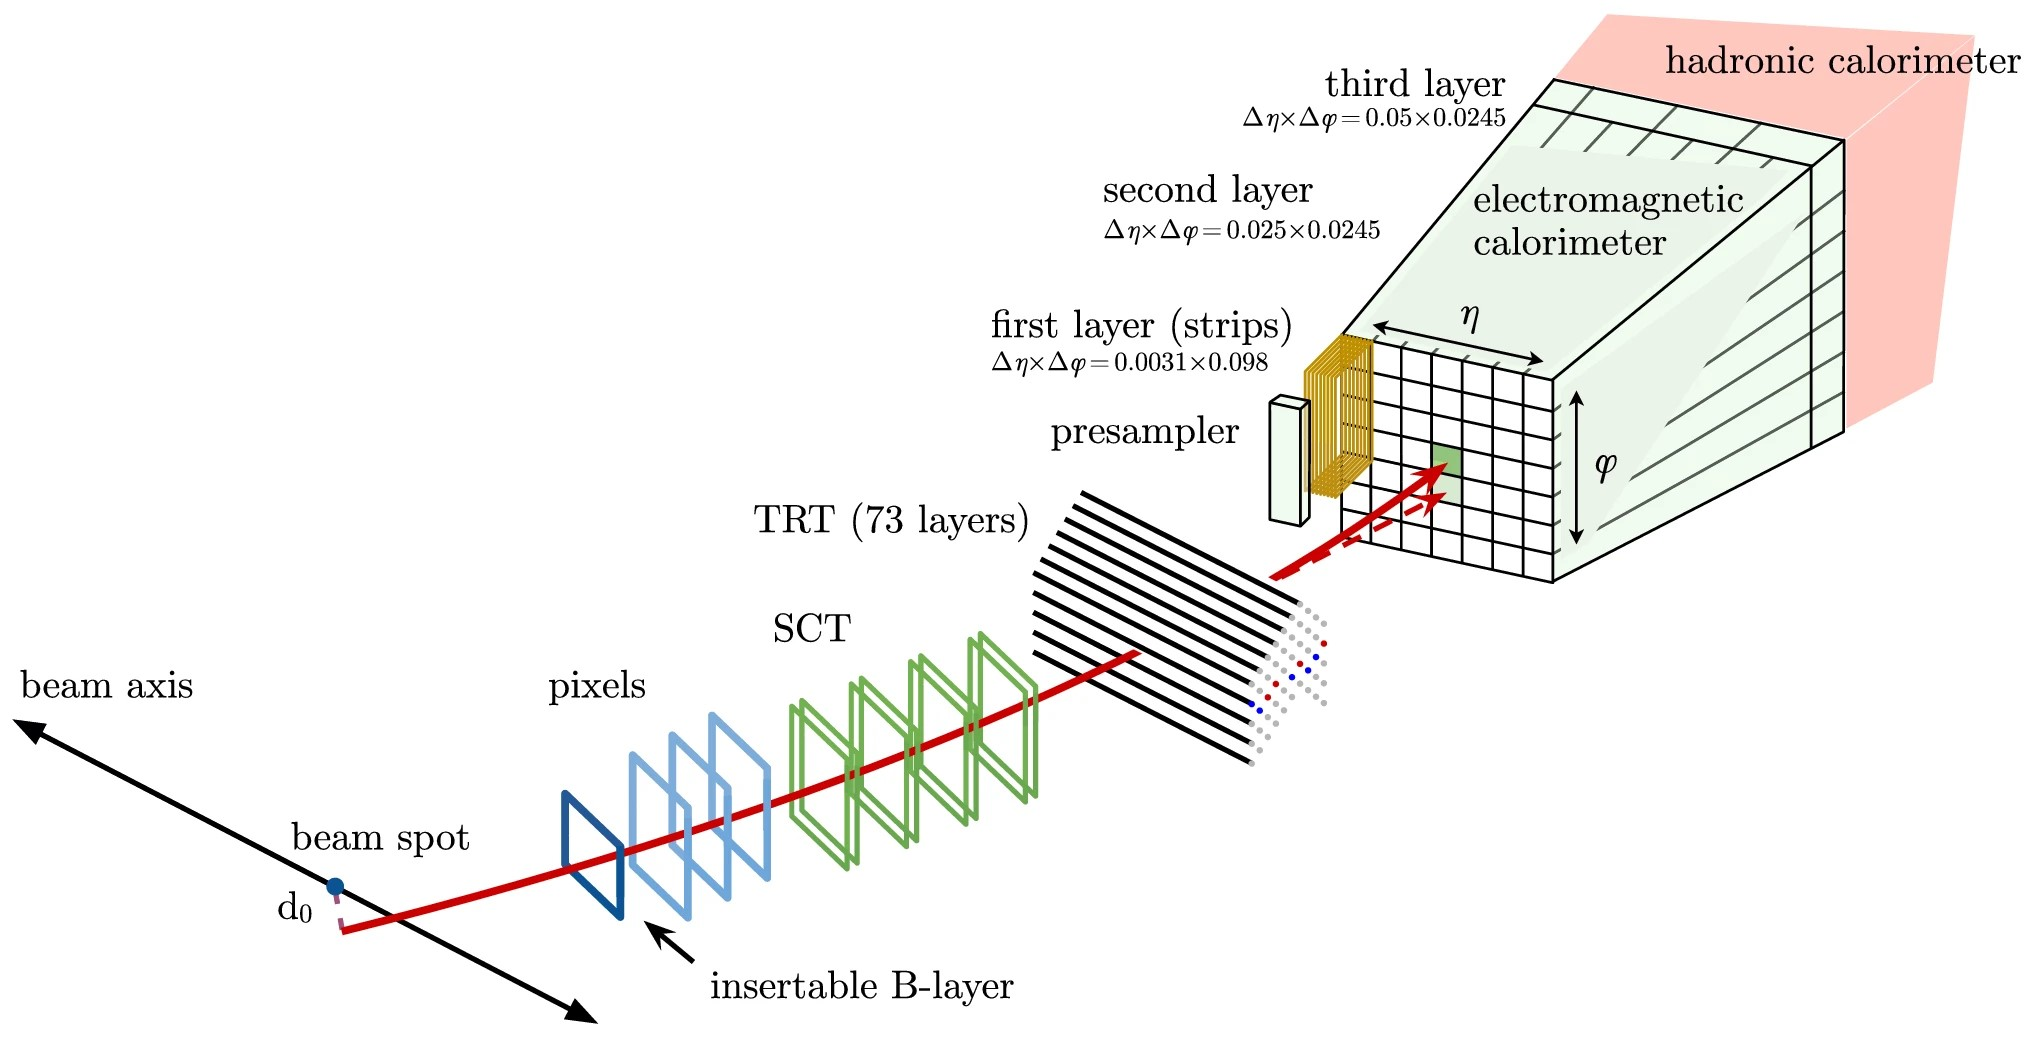
\includegraphics[width=1.0\textwidth]{Reconstruction/plots/electron.jpg}
    \caption{A schematic illustration of the path of an electron through the detector. 
    The red trajectory shows the 
    hypothetical path of an electron, which first traverses the tracking system (pixel detectors, then SCT
    and lastly the TRT) and then enters the electromagnetic calorimeter. 
    The dashed red trajectory indicates the path of a
    photon produced by the interaction of the electron with the material in the tracking system. 
    Image reproduced from Ref.~\cite{PERF-2017-01}.
        }
    \label{fig:electron_recon}
    \end{centering}
\end{figure}
The reconstruction starts from EM cluster seeding from localised energy deposits 
using a sliding-window algorithm~\cite{sliding-window}.
The $\eta \times \phi$ space of the EM is divided into \textit{towers} of 200 $\times$ 256
elements of size $\Delta\eta \times \Delta\phi$ = 0.025 $\times$ 0.025, 
consistent with the granularity of the second layer of the EM calorimeter. 
Then algorithm then ``slides'' a rectangular window of size 3 $\times$ 5 towers 
whose summed transverse energy exceeds 2.5 GeV and is a local maximum
to form a seed-cluster.
The centre of the seed moves in steps of 0.025 in 
either the $\eta$ or $\phi$ direction 
to search for localised energy deposits; 
this process is repeated until every element of the calorimeter has been covered.
To better account for the energy loss of charged particles in material,
a subsequentl fitting procedure using 
an optimised Gaussian-sum filter \cite{ATLAS-CONF-2012-047} 
is performed on tracks which are ``loosely'' matched to the EM clusters.
This matching requires the tracks and clusters to satisfy:
\begin{itemize}
    \item $|\eta_{cluster} - \eta_{track}|$ < 0.05,
\end{itemize}
and one of the two requirements:
\begin{itemize}
    \item $-0.20 < \Delta \phi < 0.05$, or
    \item $-0.10 < \Delta \phi_{res} < 0.05$,
\end{itemize}

where $\Delta\phi \equiv -q \times (\phi_{cluster} - \phi_{track})$ with 
$q$ being the charge of the particle, and 
$\phi_{cluster}$, $\phi_{track}$ and $\eta_{cluster}$, $\eta_{track}$ 
are the $\phi$, $\eta$ coordinates of
the cluster barycentre and the poisition of the track extrapolated from the 
perigee to the second layer of the calorimeter, respectively;
$\Delta \phi_{res}$ is similar to $\Delta \phi$ but with the 
momentum of the track rescaled to the energy of the cluster.
The assymmetry in the condition is to account for the energy loss
due to bremsstrahlung where tracks with negative (positive) electric charge
bend due to the magnetic field in the positive (negative) $\phi$ direction.

The matching of the fitted tracks to the candidate calorimeter seed-cluster
is the final step of electron reconstruction. 
The matching requires $-0.10 < \Delta\phi < 0.05$,
with the other alternative requirement remaining the same.
If several tracks fulfil the matching criteria, 
the track considered to be the primary electron track is selected 
using an algorithm that takes into account the distance in $\eta$
and $\phi$ between the extrapolated tracks and the cluster barycentres 
(agian, measured in the second layer of the calorimeter), 
the number of hits in the silicon detectors and in the ID layer; 
a candidate with an associated track with at least four hits in the silicon layers and no association
with a vertex from a photon conversion (photon converting into electron-positron pair) 
is considered as an electron candidate. 
However, if the primary candidate track can be matched to a secondary vertex and has no pixel hits, 
then this object is classified as a photon candidate (likely a conversion). 

A further classification is performed using the candidate electron’s $E/p$ and \pt, 
the presence of a pixel hit, and the secondary-vertex information, to determine
unambiguously whether the object is only to be considered as an electron candidate or if it should be
ambiguously classified as potentially either a photon candidate or an electron candidate.

\subsection{Identification} 
The reconstruction algorithm is very efficient in reconstructing electron,
however, this is not necessarily what is needed for many ATLAS analysis, where
they are insterested in prompt electrons. 
Prompt electrons are electrons coming from the 
primary interaction of the event, 
while non-prompt electrons may come from
the semileptonic decays of heavy quarks or from photon conversion.
Other objects such as hadrons can be 
mis-reconstructed as electrons as well.
This necessitates the identification of prompt electrons, 
making use of the differences between prompt electrons 
and non-prompt electrons/mis-reconstructed electrons.
A multivariate likelihood technique, taking advantages of the correlations
among the variables describing the differences,
is employed to select prompt electrons~\cite{PERF-2017-01}.
The input variables to the likelihood 
describe the following characteristics: 
a) shower shape, b) properties of the track, c) matching
of the track and clusters.

To quantify the performance of the identification, 
the identification efficiency is measured, 
which represents the probability of
a true prompt electron passing the identification requirements.
Different cuts are applied on the final discriminant
to define \textit{working points} (WP), which can specify 
the identification efficiency, as a function of $E_T$ or $\eta$ of the electron. 
Three WPs, \textit{Loose}, \textit{Medium} and \textit{Tight} are defined.
Each WP is
utilising a separate mulitvariate discriminant formed from 
a different selection of discriminating variables, 
and applying a different requirement on the resulting discriminant output.
% places a different requirement on final discriminant 
% made with a different set of variables. 
An example of the electron identification efficiency 
is shown in Figure~\ref{fig:electron_ID}.
\begin{figure}[bht]
    \begin{centering}	
    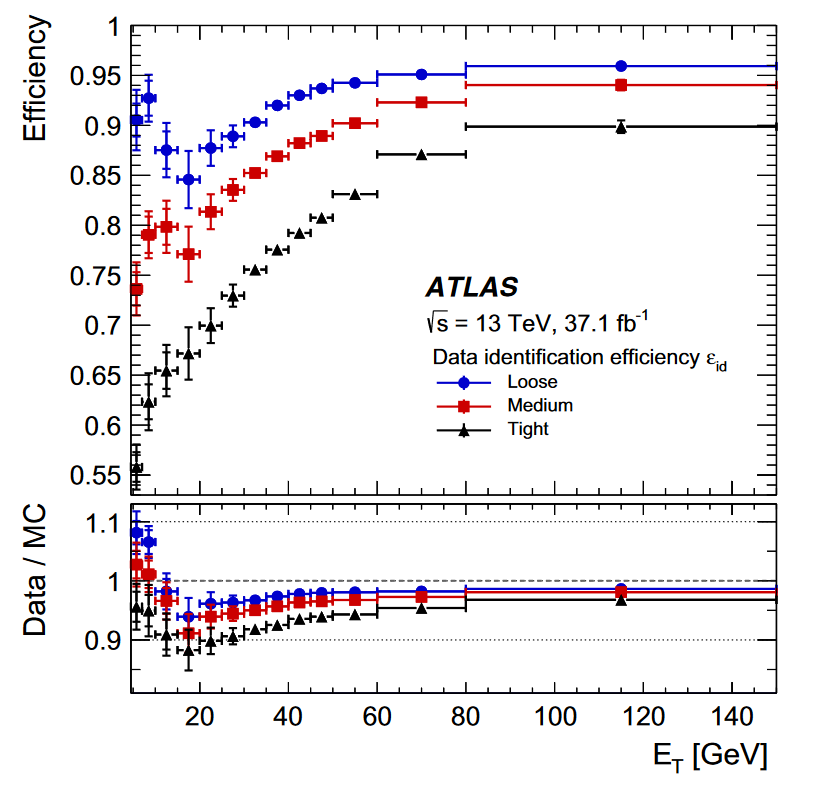
\includegraphics[width=0.45\textwidth]{Reconstruction/plots/electrond_ID1.png}
    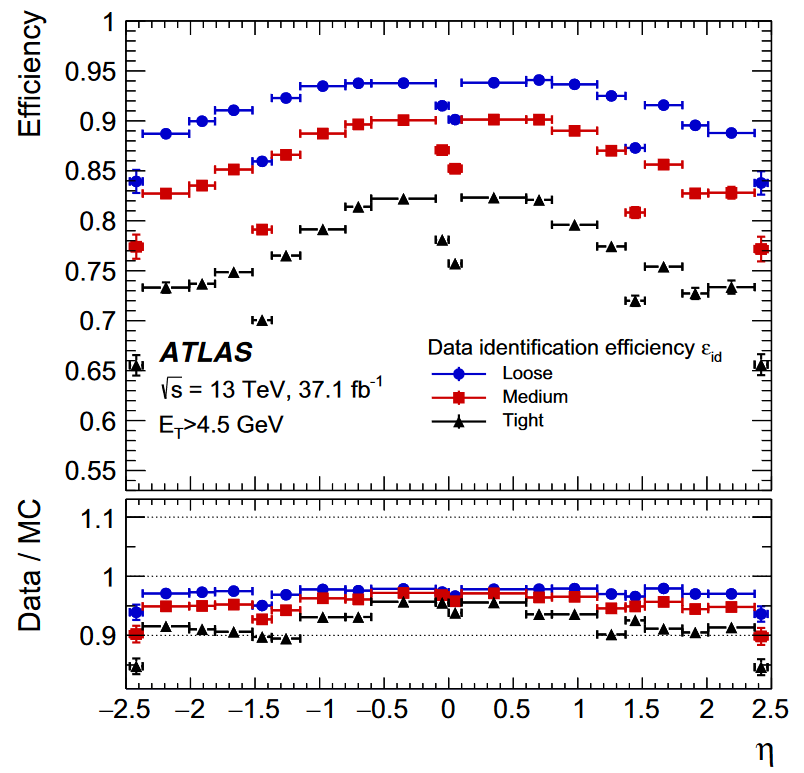
\includegraphics[width=0.45\textwidth]{Reconstruction/plots/electrond_ID2.png}
    \caption{Measured electron identification efficiencies in $Z \rightarrow ee$
    events for the `Loose' (blue circles), `Medium' (red squares), 
    and `Tight' (black triangles) WPs as a function of $E_T$ (left) and $\eta$ (right). 
    The vertical uncertainty bars (barely visible because they are small) 
    represent the statistical (ID) and total (outer bars) uncertainties. 
    For both plots, the bottom panel shows the data-to-simulation
    ratios. Reproduced from Ref.~\cite{PERF-2017-01}.}
    \label{fig:electron_ID}
    \end{centering}
\end{figure}

In addition, many analyses further require the electron to pass
some \textit{isolation} requirements.
Isolation is built exploiting a characteristic signature 
of the prompt electrons that 
there is relatively little activity surrounding 
the prompt electrons, as compared to non-prompt electrons~\cite{EGAM-2018-01}. 
For the electron isolation, 
four WPs: \textit{Gradient}, \textit{HighPtCaloOnly}, \textit{Loose} and \textit{Tight} 
are defined, each targeting a fixed value of isolation efficiency
or imposing fixed requirement on the isolation variables. 

In the analysis presented in Chapter~\ref{sec:search for dihiggs} 
the `Loose' identification WP is used, which, in combination with 
additional track hit requirements, provides an electron efficiency of 95\%.
The electron candidates are also required to have \pt\ > 7 GeV and $|\eta|$ < 2.47.
Further cuts are used to define signal electrons, as defined in 
section~\ref{sec:DiHiggs:selection}. 
% with additional requirements on the electron 
In addition, the electron candidates are required
to pass the `Loose' isolation WP which has an efficiency of 99\%. 
The isolation requirement is also 
inverted to provide control regions for estimating backgrounds, 
as described in section~\ref{sec:DiHiggs:lephadfake}.
% , achieving 99\% efficiency 
% that is constant across the entire \pt\ spectrum.
In the FTAG calibration effort presented in Chapter~\ref{sec:FTAG} 
the `Medium' identification WP is used, where the electron efficiency is roughly
85\%, 
with additional requirements on the electron \pt\ > 27 GeV and $|\eta|$ < 2.47
(while unlike requirements in Chapter~\ref{sec:search for dihiggs},
no further cuts are applied).
Electrons are required to pass the `Gradient' isolation WP,
designed to give an efficiency of 90\% at \pt\ = 25 GeV and 99\% at \pt\ = 60 GeV.
% The different requirements in the two chapters 
% is the result of different signal targeted and hence different 
% purity and phase space is needed. 
% The `Loose' WP features variables most useful for discrimination against light-flavour jets. 
% In the `Medium' and `Tight' regimes, additional variables are added for further rejection 
% of heavy-flavour jets and photon conversions. 
% Although different variables are used for the different selections, a sample of electrons selected using a tighter LH
% is a subset of the electron samples selected using the looser LH to a very good approximation

% \textit{isolation} is built, usually by 
% summing the transverse energies of clusters in the calorimeter 
% or the transverse momenta of tracks in a cone of radius
% $\Delta R$ around the direction of the electron
% candidate, excluding the candidate itself

% The inputs to the likelihood include measurements from the tracking system, the
% calorimeter system, and quantities that combine both tracking and calorimeter information.
% The main advantages using the likelihood-based method comparing with 
% a selection-criteria-based (so-called ``cut-based'') identification is that
% a prompt electron may fail the cut-based identification because it
% does not satisfy the selection criterion for a single quantity, 
% while in the likelihood-based selection this electron can
% still satisfy the identification criteria, 
% because the likelihood combines the information of all of the discriminating variables.
% The final discriminant produced by the likelihood method is used to define 
% three \textit{working points} (WP), which are cuts in the final discriminant 
% identifying the different identification efficiencies. 






\section{Muons}
The characteristic behaviour of a muon in the detector is a particle
ionising minimally. 
The muon reconstruction is done taking advantage of this feature, 
with information from the ID and MS tracking detectors being combined, 
while information from the calorimeters is also used
to account for cases of
large energy loss in the calorimeters, and for MS-independent
tagging of ID tracks as muon candidates in regions of limited MS
coverage~\cite{CERN-EP-2020-199}.
On the orther hand, 
the muon identification is performed by applying 
quality requirements that suppress background, 
mainly from pion and kaon decays, that 
% , while selecting prompt muons with high efficiency.
muon candidates oftenly leave a distinctive “kink” topology 
in the reconstructed track, and hence degrade the quality of the track. 


\subsection{Reconstruction}
The muon reconstruction consists of two steps. 
The first step is to reconstruct the stand-alone track in the MS,
followed by reconstruction with complete detector information.
The first step of reconstruction starts with the identification 
of short straight-line local track segments reconstructed 
from hits in an individual MS \textit{stations} (layers). 
At least two of these segments are then required
to build preliminary track candidates, 
with information from precision measurements in the bending plane 
and measurements of the second coordinate from 
the MS trigger detectors to create three-dimensional track candidates. 
A global $\chi^2$ fit of the muon trajectory 
through the magnetic field is performed,
outlier hits are removed and hits along the trajectory that
were not assigned to the original track candidate are added.
Finally, the tracks are fitted again with the updated hits information,
and ambiguities are resolved by removing tracks
that share a large fraction of hits with higher-quality tracks.

The second step of reconstruction is to combine the track candidates 
with the complete information of all sub-detectors.
The reconstruction proceeds according to five main
reconstruction strategies, leading to the corresponding muon
types: 
\begin{itemize}
\item \textit{combined muons} 
are identified by matching 
MS tracks to ID tracks and performing a combined track fit 
based on the ID and MS hits, taking into account the energy loss in the
calorimeters, in the region $|\eta|$ < 2.5.
\item \textit{Inside out muons} 
are reconstructed in the region $|\eta|$ < 2.5 using a complementary
inside-out algorithm, which extrapolates ID tracks to the MS
and searches for at least three loosely-aligned MS hits. The
ID track, the energy loss in the calorimeters and the MS hits
are then used in a combined track fit. 
% This algorithm does
% not rely on an independently reconstructed MS track, and
% therefore recovers some efficiency.
\item \textit{Muon-spectrometer extrapolated muons} are muons 
reconstructed when a MS track cannot be matched to an ID track. 
Its parameters are extrapolated to the beamline and used to define an
Muon-spectrometer extrapolated muon. 
Such muons are used to extend the acceptance
outside that of the ID ($|\eta|$ <2.5), thus exploiting the full MS 
coverage up to $|\eta|$ = 2.7.
\item \textit{segment-tagged muons} 
are identified by requiring that an ID track
extrapolated to the MS satisfies tight angular matching
requirements to at least one reconstructed MS segment, 
in the $|\eta|$ < 2.5 region. 
% A successfully-matched ID track is identified as a muon candidate, 
% and the muon parameters are taken directly from the
% ID track fit.
\item \textit{calorimeter-tagged muons} 
are identified by extrapolating ID
tracks through the calorimeters to search for energy deposits
consistent with a minimum-ionising particle, in the region $|\eta|$ < 0.1.
\end{itemize}
\subsection{Identification}

As a consequence, it is expected that the fit quality of the resulting combined track 
will be poor and that the momentum measured in the ID and MS may not be compatible~\cite{PERF-2015-10}. 
Therefore, a set of requirements are applied on the
number of hits in the different ID subdetectors and different
MS stations, on the track fit properties, 
and on variables that test the compatibility of the individual measurements 
in the two detector systems~\cite{CERN-EP-2020-199}.
A given set of requirements for each of the muon types defined above
is referred to as working point (WP).
The main metrics considered for designing the WPs are 
the selection efficiency and purity in simulation,
where the prompt muon efficiency of a selection WP 
represents the probability that a real prompt muon traversing the detector 
is reconstructed as a muon and satisfies the WP; the purity
of a selection WP is one minus the hadron misidentification
rate (the fraction of light hadrons reconstructed as muons 
and satisfying the WP).
Three standard selection WPs: \textit{Loose},
\textit{Medium}, and \textit{Tight} are designed to 
cover the majority of physics analysis, while
two additional WPs, \textit{High-\pt} and \textit{Low-\pt},
are designed to accommodate the analyses targeting extreme 
phase space. 
An example of the reconstruction and isolation efficiency of muon is 
shown in Figure~\ref{fig:muon_ID}.
\begin{figure}[bht]
    \begin{centering}	
    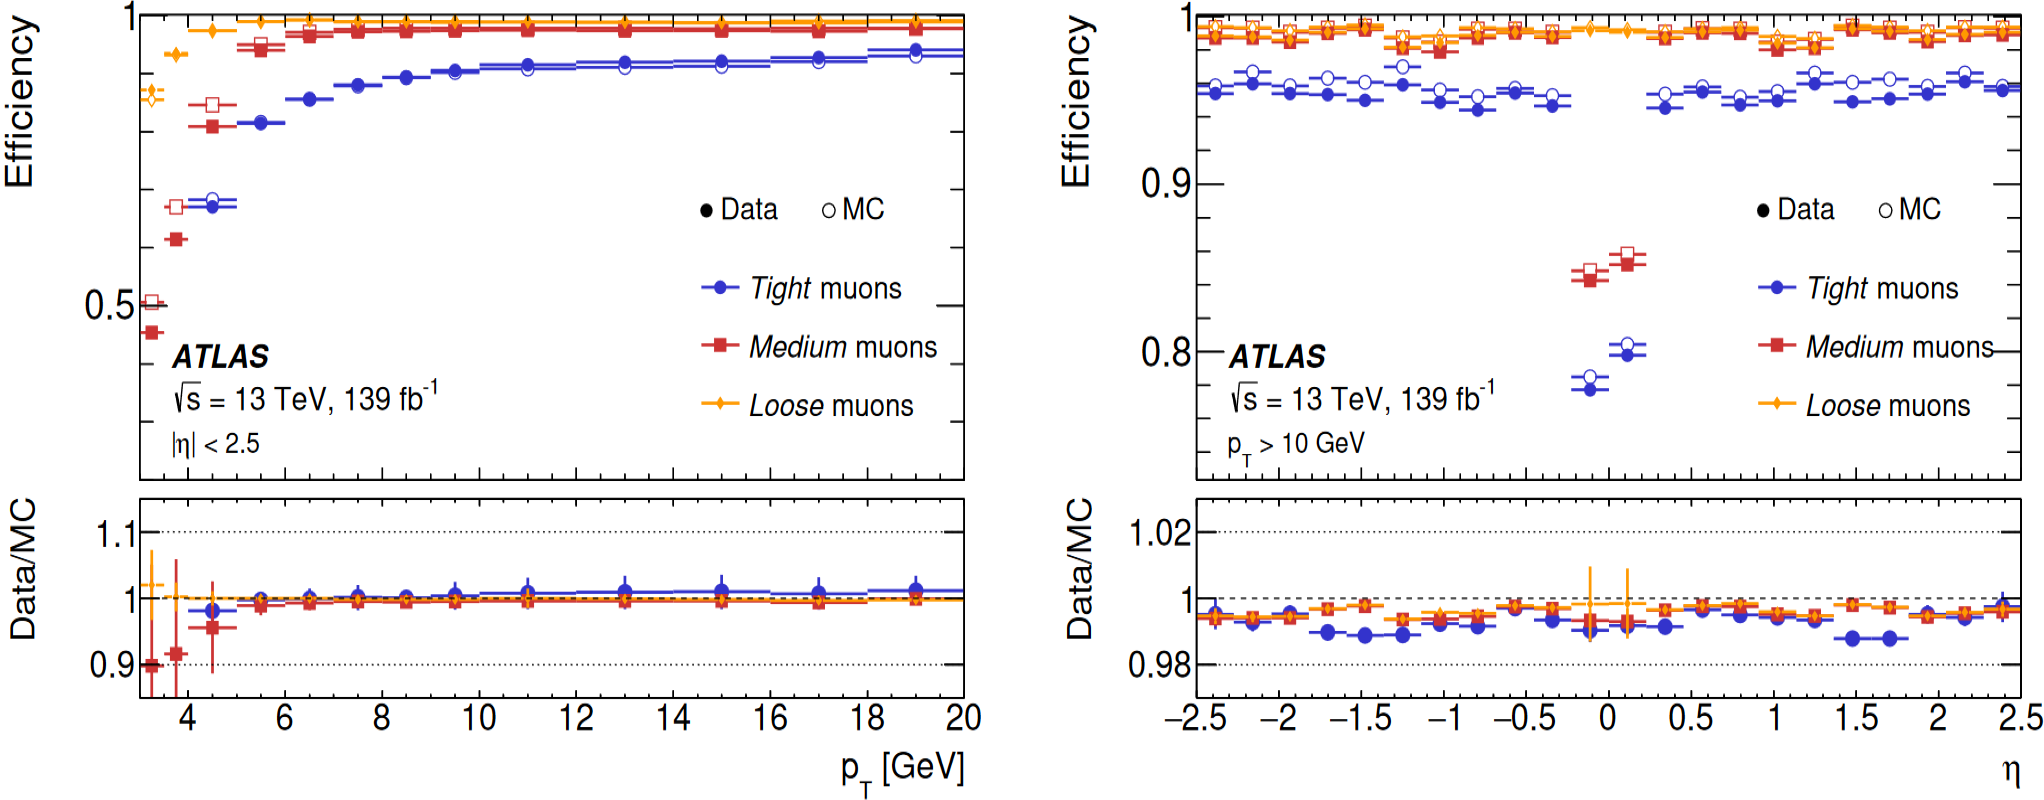
\includegraphics[width=1.0\textwidth]{Reconstruction/plots/muon_ID.png}
    \caption{
        Muon reconstruction and identification efficiencies for the Loose, Medium, and Tight criteria. 
        The left plot shows the efficiencies measured in $J/\psi \rightarrow \mu\mu$ events as function of \pt. 
        The right plot displays the efficiencies measured in $Z \rightarrow \mu\mu$ events as a function of $\eta$, 
        for muons with \pt\ > 10 GeV. The predicted efficiencies are depicted as open markers, 
        while filled markers illustrate the result of the measurement in collision data. 
        The statistical uncertainty in the efficiency measurement is smaller than the size of the markers, 
        and thus not displayed. The panel at the bottom shows the ratio of the measured to predicted efficiencies, 
        with statistical and systematic uncertainties.
        Reproduced from Ref.~\cite{CERN-EP-2020-199}.}
    \label{fig:muon_ID}
    \end{centering}
\end{figure}

In Chapter~\ref{sec:search for dihiggs}, muons are selected
with \pt\ > 7 GeV and $|\eta|$ < 2.7, and passing the `loose' 
identification criteria with an efficiency of about 95\%, 
as well as the `pflowLoose\_VarRadIso' 
isolation criteria~\cite{MuonWP} with an efficiency of 
roughly 97\%. 
(further cuts are applied to define signal muons, 
as defined in section~\ref{sec:DiHiggs:selection});
while in Chapter~\ref{sec:FTAG} muons are selected
with \pt\ > 27 GeV and $|\eta|$ < 2.5, and passing the `medium' 
identification criteria as well as a track-based isolation criteria, 
`TightTrackOnly' with an efficiency of around 94\%~\cite{CERN-EP-2020-199} 
(with no further cuts applied).
